% simdoc.tex V3.0, 30 March 2010

\documentclass[times]{simauth}

\usepackage{moreverb}

%\usepackage[T1,mtbold]{mathtime} % commented by ShareLaTeX Team because of compilation errors

\usepackage[
%dvips, % commented by ShareLaTeX Team because of compilation errors
colorlinks,bookmarksopen,bookmarksnumbered,citecolor=red,urlcolor=red]{hyperref}

\usepackage[utf8]{inputenc}
\usepackage[T1]{fontenc}
\usepackage[spanish]{babel}
\usepackage{wrapfig}
\usepackage{framed}
\usepackage{upquote}
\usepackage{epigraph}
\usepackage{makeidx}
\graphicspath{ {images/} }

%\newcommand{\mysmall}{\fontsize{7.5pt}{8pt}\selectfont}

%\newcommand\BibTeX{{\rmfamily B\kern-.05em \textsc{i\kern-.025em b}\kern-.08em
%T\kern-.1667em\lower.7ex\hbox{E}\kern-.125emX}}

\def\volumeyear{2010}

\begin{document}

%\runninghead{A.~N.~Other}

\title{
    {\fontfamily{ppl} \fontsize{30}{1} \selectfont{
        Tarea \#3:\\ Falacias de razonamiento en medios de comunicación nacional}
    }
}

\author{
    {\fontfamily{ppl} \fontsize{14}{1} \selectfont{
        Carlos Martín Flores González \\
        Raquel Rodríguez Chaves}
    }
}

%\address{John Wiley \& Sons, Ltd, The Atrium, Southern Gate, Chichester,
%West Sussex, PO19~8SQ, UK}
%
%\corraddr{Journals Production Department, John Wiley \& Sons, Ltd,
%The Atrium, Southern Gate, Chichester, West Sussex, PO19~8SQ, UK.}

%\begin{abstract}
%This paper describes the use of the \LaTeXe\ \textsf{simauth.cls}
%class file for setting papers for \emph{Statistics in Medicine}.
%\end{abstract}

%\keywords{class file; \LaTeXe; \emph{Statist.\ Med.}}

\maketitle

\tableofcontents

\newpage
\section{Falacia 1: Diputado equipara Costa Rica con la Alemania Nazi}

\begin{figure}[h]
    \centering
    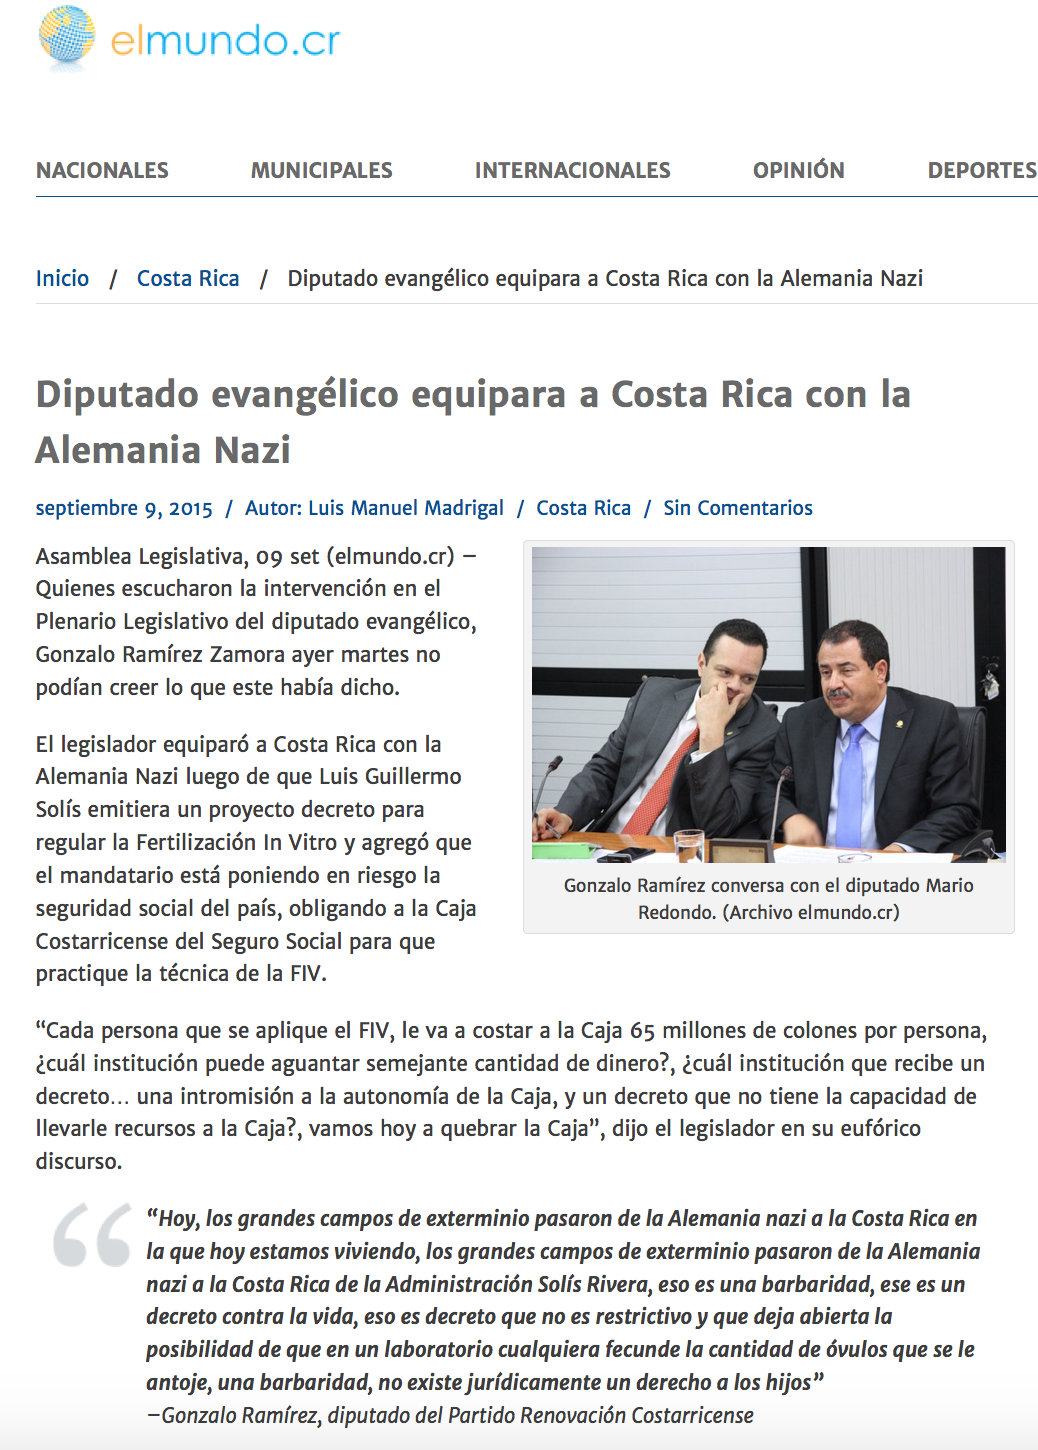
\includegraphics[width=15cm]{costarica-nazi-fiv}
    \captionof{figure}{Captura de pantalla de la noticia}
    \label{fig:falacia1}
\end{figure}

\newpage

\begin{table}[h!]
    \begin{tabular}{ll} 
        \toprule[1.5pt]
        Fuente & Periódico \href{http://elmundo.cr}{elmundo.cr}\\
        \midrule[0.5pt]
        Fecha  & 9 de setiembre 2015\\
        \midrule[0.5pt]
        Falacia & Palabras emotivas \\
        \bottomrule[1.5pt]
    \end{tabular} 
\end{table}

El legalización de la técnica de Fertilización in Vitro (FIV) ha resultado ser un tema muy polémico en nuestro país, principalmente en la asamblea legislativa en donde un pequeño grupo de diputados de partidos conservadores se oponen a la utilización de esta técnica aduciendo que atenta contra la vida humana.

En su discurso de la sesión del día martes 8 de setiembre del 2015, el diputado evangélico Gonzalo Ramírez Zamora, un claro opositor del FIV, llegó a comparar a Costa Rica con la Alamania Nazi diciendo que: \textit{``Hoy, los grandes campos de exterminio pasaron de la Alemania nazi a la Costa Rica en la que hoy estamos viviendo, los grandes campos de exterminio pasaron de la Alemania nazi a la Costa Rica de la Administración Solís Rivera, eso es una barbaridad, ese es un decreto contra la vida, eso es decreto que no es restrictivo y que deja abierta la posibilidad de que en un laboratorio cualquiera fecunde la cantidad de óvulos que se le antoje, una barbaridad, no existe jurídicamente un derecho a los hijos''}.

En su discurso el diputado Ramírez hace un claro uso de palabras emotivas con el fin de despertar sentimientos negativos ante la posible aprobación de esta técnica, de esta forma tanto diputados presentes, seguidores de su partido y público en general podrían llegar a crear sentimientos de miedo u odio con el fin de generar mayor oposición.

\noindent Dirección: \href{http://www.elmundo.cr/costarica/diputado-equipara-costa-rica-la-alemania-nazi-decreto-la-fiv/}{http://www.elmundo.cr/costarica/diputado-equipara-costa-rica-la-alemania-nazi-decreto-la-fiv/} \\
Discurso del diputado Ramírez: \href{https://www.youtube.com/watch?v=cK6AeaFB1Co}{https://www.youtube.com/watch?v=cK6AeaFB1Co}\\


\newpage
\section{Falacia 2: Periodistas cuestionan a la costarricense del milagro sobre los incrédulos}

\begin{figure}[h]
    \centering
    
\includegraphics[width=15cm]{floribeth-mora-milagro}
    \captionof{figure}{Detalle de la noticia sobre el cuestionamiento del milagro de Floribeth Mora}
    \label{fig:falacia2}
\end{figure}

\newpage

\begin{table}[h!]
    \begin{tabular}{ll} 
        \toprule[1.5pt]
        Fuente & Periódico La Nación\\
        \midrule[0.5pt]
        Fecha  & 24 de abril 2014\\
        \midrule[0.5pt]
        Falacia & Peso de la prueba, Inexplicado vs Inexplicable \\
        \bottomrule[1.5pt]
    \end{tabular} 
\end{table}


En el año 2011 Floribeth Mora, una ama de casa de 50 años residente en La Unión de Cartago, fue diagnosticada con un aneurisma en el lado izquierdo del cerebro. Luego de ser internada y de tener un estado de salud crítica, el aneurisma desapareció sin dejar rastro lo cual salvó Floribeth de la muerte. Ella aduce de que fue curada gracias a la intervención del fallecido Papa Juan Pablo II, el cual se le manisfestó por sueños. Esta historia logró trascender hasta llegar al Vaticano en donde luego de un estudio determinaron el caso de Floribeth calificaba como de milagro y gracias al mismo se concedió la beatificación del Papa.

En entrevistas y conferencias de prensa Floribeth manifestó de que: \textit{``Mi interés no está en convencer a los incrédulos. Dios me escogió y por su voluntad es que estoy acá. Lo importante es que esta loca, que ellos llaman, está sana''}. En estas declaraciones queda claro de que no se proporciona ninguna prueba que pueda ser refutada. Lo que se provee más bien es una especie de ``salida fácil'' ante los eventos por los cuales ella pasó. Se fabrica una explicación ``mágica'' que elimina cualquier proceso de razonamiento.

Esta noticia está disponible en:  \href{http://www.nacion.com/nacional/religion/Periodistas-cuestionan-costarricense-milagro-incredulos_0_1410459070.html?print=1}{http://www.nacion.com/nacional/religion/Periodistas-cuestionan-costarricense-milagro-incredulos\_0\_1410459070.html?print=1}

\newpage
\section{Falacia 3: Jefa de prensa OIJ ganará ¢53 millones sin trabajar}

\begin{figure}[h!]
    \centering
    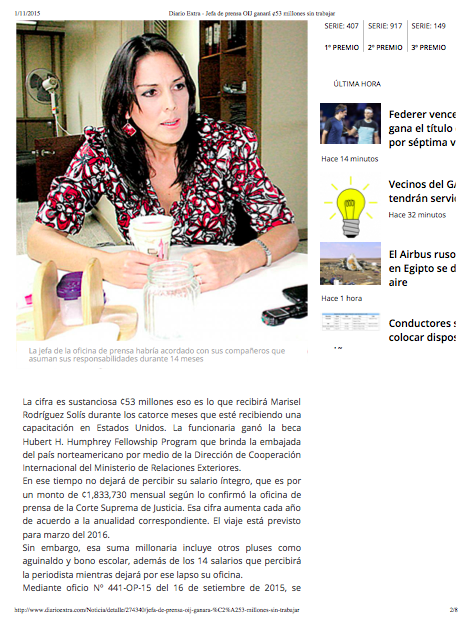
\includegraphics[width=15cm]{noticiaJefaOIJ}
    \captionof{figure}{Captura de pantalla noticia: Jefa de prensa OIJ ganará ¢53 millones sin trabajar}
    \label{fig:falacia3}
\end{figure}

\newpage

\begin{table}[h!]
    \begin{tabular}{ll} 
        \toprule[1.5pt]
        Fuente & Periódico La Extra\\
        \midrule[0.5pt]
        Fecha  & 01 de noviembre 2015\\
        \midrule[0.5pt]
        Falacia & Ad populum, palabras emotivas, falsas analogías. \\
        \bottomrule[1.5pt]
    \end{tabular} 
\end{table}

El artículo está redactado de una manera manipuladora para incentivar sentimientos de odio en la población.  El uso de frases como: “sin trabajar”, “suma millonaria”, “todo pago”, “no cumple requisitos” dan una connotación negativa de a noticia desde el título y  sesgan la opinión del lector.

Las misma noticias podría haberse presentado de manera positiva con solo cambiar la redacción. Por ejemplo haber incluyendo palabras como: ganar, oportunidad, orgullo y equidad de genero hubiesen generado en el lector sentimientos diferentes. 
Sería idean sería que las noticias se redactaran de manera imparcial, y permitieran a los lectores decidir por si mismo su opinión. 

Esta noticia está disponible en: http://www.diarioextra.com/Noticia/detalle/274340/jefa-de-prensa-oij-ganara-%C2%A253-millones-sin-trabajar


\newpage
\section{Falacia 4: ¿Qué probabilidad de éxito dan los expertos a la Selección de Costa Rica}

\begin{figure}[h!]
    \centering
    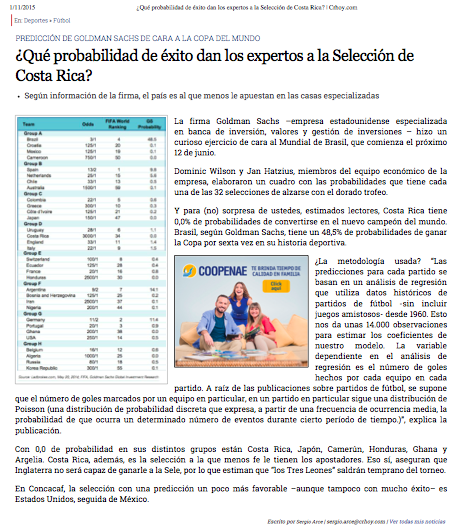
\includegraphics[width=15cm]{exitoSeleccion}
    \captionof{figure}{Captura de pantalla noticia: ¿Qué probabilidad de éxito dan los expertos a la Selección de
Costa Rica?}
    \label{fig:falacia4}
\end{figure}



\newpage
\begin{table}[h!]
    \begin{tabular}{ll} 
        \toprule[1.5pt]
        Fuente & Periódico CRHoy\\
        \midrule[0.5pt]
        Fecha  & 28 de mayo 2014\\
        \midrule[0.5pt]
        Falacia & Post Hoc, Ergo Propter Hoc \\
        \bottomrule[1.5pt]
    \end{tabular} 
\end{table}

El análisis que utilizan es el siguiente: como siempre les va mal = les va a ir mal.

Basar la investigación es el número de goles hechos por cada equipo en el pasado no es puede determinar la probabilidad de ganar de un equipo en el estado actúa. No existe correlación, se trata más bien de una secuencia de eventos independientes.

Las razón reales de porque un equipo de futbol ha tenido un mal desempeño en el pasado no son analizadas. Razones como: mala condición física, poco entrenamiento, limitaciones económicas, mal entrenador, desmotivación entre otras,  pueden cambiar y un equipo de futbol de repente puede pasar de malo a bueno. De manera contraria un equipo de futbol puede de repente pasar de bueno a malo. Por lo tanto, consideramos que este estudio no tiene valor. 

Esta noticia está disponible en: http://www.crhoy.com/cuantas-posibilidades-dan-los-expertos-a-la-seleccion-de-costa-rica-v2h3h7x/

\newpage
\section{Falacia 5: Lorem Ipsum}

\section{Falacia 6: Lorem Ipsum}

\section{Falacia 7: Lorem Ipsum}

\section{Falacia 8: Lorem Ipsum}

\section{Falacia 9: Lorem Ipsum}

\section{Falacia 10: Lorem Ipsum}

\section{Falacia 11: Lorem Ipsum}

\section{Falacia 12: Lorem Ipsum}


\begin{thebibliography}{9}

\bibitem{R1} Kopka~H, Daly~PW. 2003. \emph{A Guide to \LaTeX} (4th~edn).
Addison-Wesley.

\bibitem{R2} Lamport~L. 1994. \emph{\LaTeX: a Document Preparation System} (2nd~edn).
Addison-Wesley.

\bibitem{R3} Mittelbach~F, Goossens~M. 2004. \emph{The \LaTeX\ Companion}
(2nd~edn). Addison-Wesley.
\end{thebibliography}
\end{document}

